\section{Method}

\begin{figure}
	\centering
	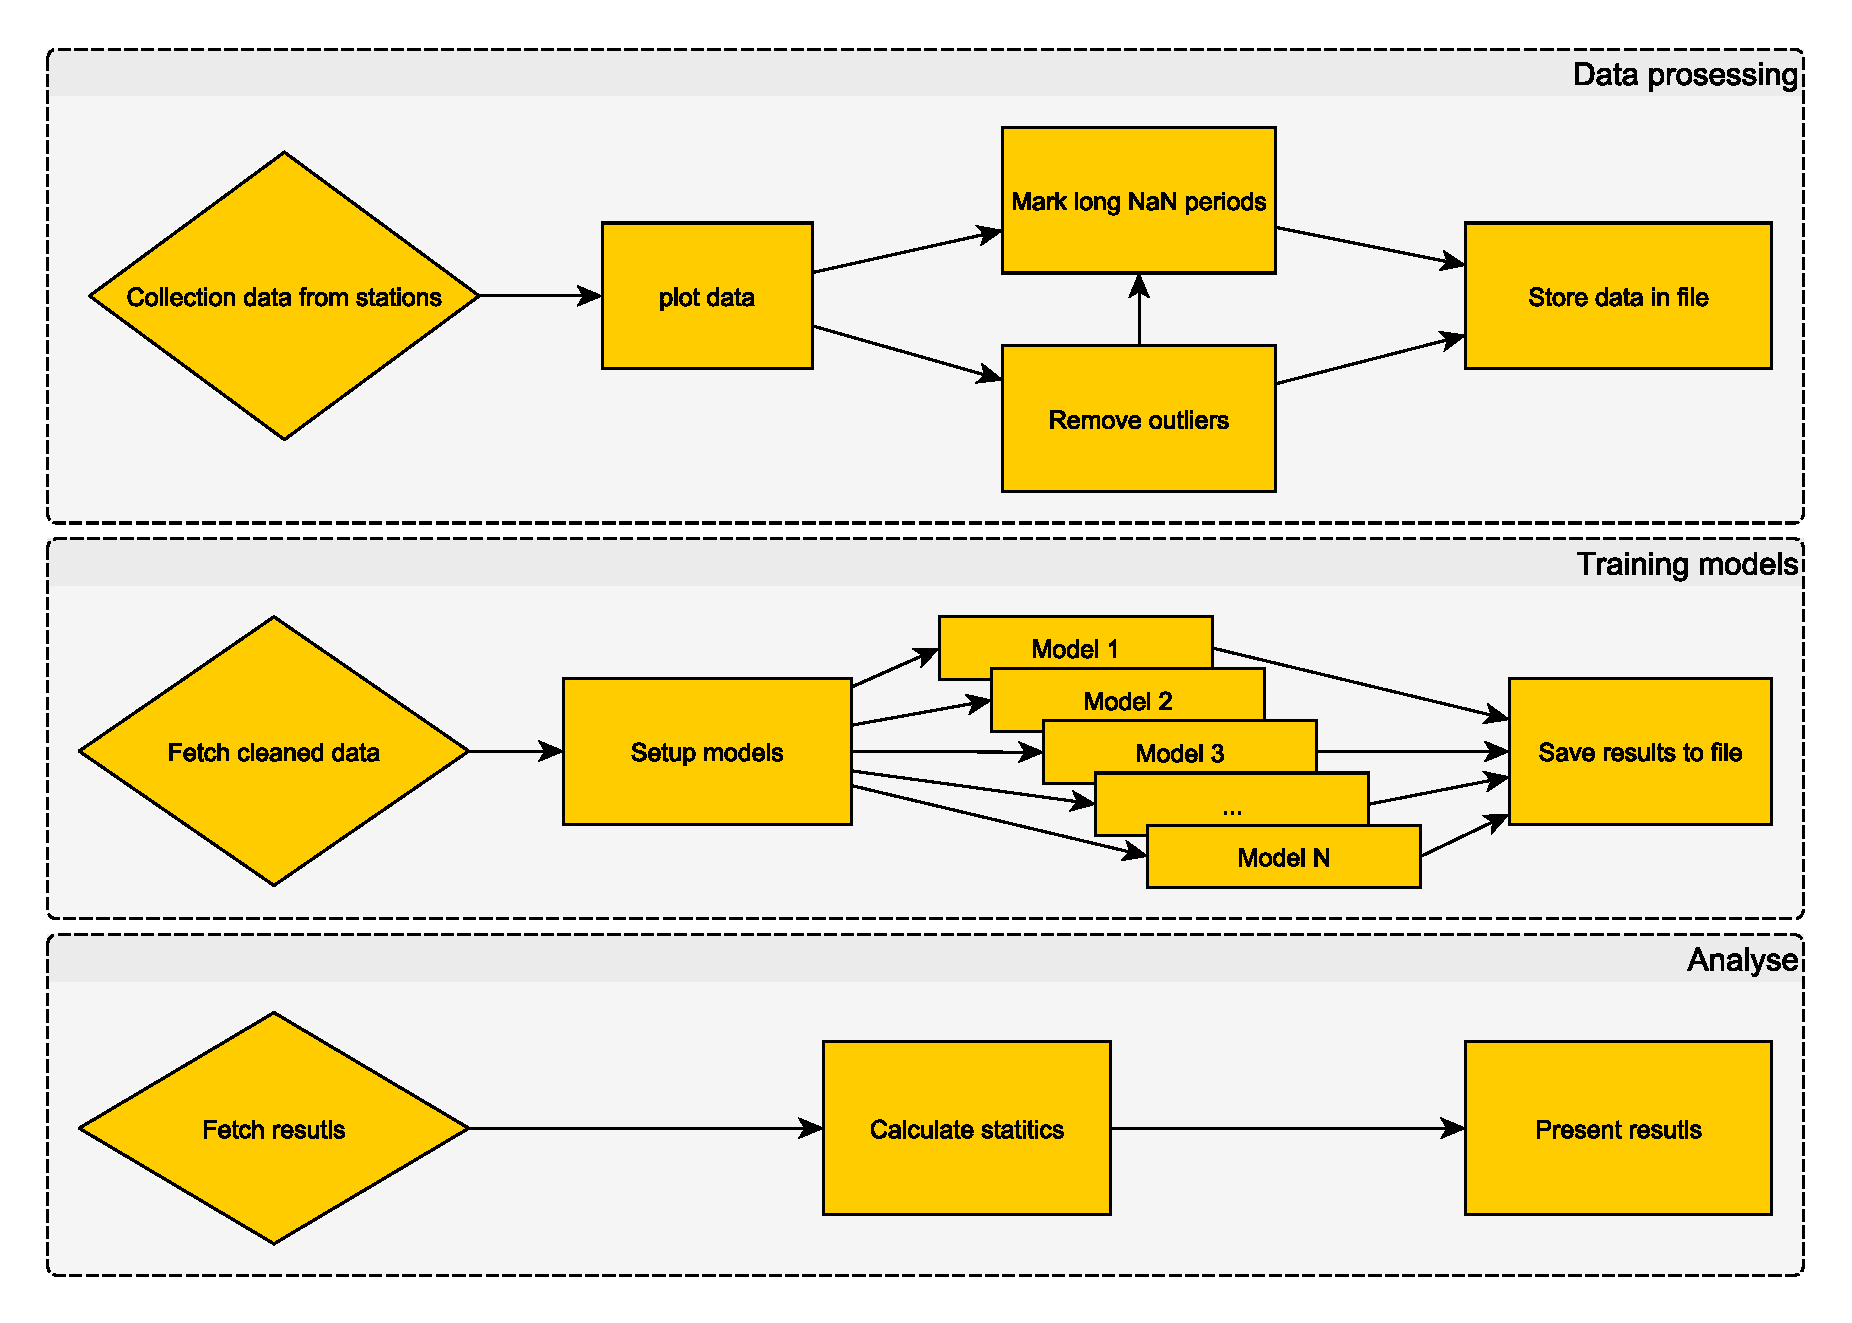
\includegraphics[width=0.7\linewidth]{figures/progress_diagram}
	\caption[Diagram sketching three procedures used in this study.]{A surface level diagram of the methodology.}
	\label{fig:progressdiagram}
\end{figure}

\subsection{Source of data}

For this comparative study the following data sources will be used

\begin{enumerate*}
	\item \acrfull{ac:nibio}
	\item \acrfull{ac:kilden}
	\item \acrfull{ac:met}
\end{enumerate*}

\subsection{Dataset}

The dataset is chosen from four regions in Norway; Innlandet, Vestfold, Trøndelag, and Østfold. From each region are four stations picked shown in table \ref{tab:station:names}
\begin{table}[h]
	\begin{adjustwidth}{-1in}{-1in}
		\centering
		\begin{tabular}{llrlrrrr}
			\hline Region&Name&ID&Drain type&MET name& Latitude&Longdetude&Altitude [m.a.s.l.]\\\hline
			Innlandet&Apelsvoll&11& Self-drained&SN11500&60,70024&10,86952&262\\
			Innlandet& Fåvang&17& Self-drained&SN13150&61,45822&10,18720&184\\
			Innlandet& Ilseng&26& Self-drained&SN12180&60,80264&11,20298&182\\
			Innlandet& Kise&27& Saturated&SN12550&60,77324&10,80569&129\\
			Trøndelag& Kvithamar&57& Saturated&SN69150&63,48795&10,87994&28\\
			Trøndelag& Frosta&15& Self-drained&SN69655&63,56502&10,69298&18\\
			Trøndelag& Mære&34& Self-drained&SN71320&63,94244&11,42527&59\\
			Trøndelag& Rissa&39& Saturated&SN71320&63,58569&9,97007&23\\
			Vestfold& Lier&30& Saturated&SN19940&59,79084&10,25962&38\\
			Vestfold& Sande&42& Saturated&SN26990&59,61620&10,22339&35\\
			Vestfold& Tjølling&50& Self-drained&SN27780&59,04641&10,12513&19\\
			Vestfold& Ramnes&38& Saturated&SN27315&59,38081&10,23970&39\\
			Østfold& Rakkestad&37& Saturated&SN3290&59,38824&11,39042&102\\
			Østfold& Rygge&41& Self-drained&SN17380&59,39805&10,75427&35\\
			Østfold& Tomb&52& Saturated&SN17050&59,31893&10,81449&12\\
			Østfold& Øsaker&118& Saturated&SN3370&59,31936&11,04221&45\\\hline
		\end{tabular}
	\end{adjustwidth}
	\caption[Staion information for each station/w location and MET-ID]{Station information from stations used in this study. The MET names was found by looking at the coordinates of the station and finding the closest MET station coordinates. \acrshort{ac:masl} stands for \acrlong{ac:masl}. The ID will be used in the text, tables, and figures for convenience and it was used in the code for something.}
	\label{tab:station:names}
\end{table}

% ™. These parameters were meticulously compiled from the Long-term Meteorological Trends (LMT) database, ensuring a robust dataset for evaluating temporal soil and air temperature patterns. This rich dataset provides valuable insights into the thermal dynamics of soil and air, which are essential for a multitude of ecological and agricultural applications.

The dataset created from all stations, spanning the period of 1st of March to 31st of October, annually from 2016 through 2022. This timeframe was selected to capture the critical growing seasons across various regions. The specific features extracted for analysis include the mean hourly soil temperature at a depth of 10cm (denoted as TJM10), the mean hourly soil temperature at 20cm (TJM20), and the mean hourly air temperature measured at 2 meters above ground level. These parameters were collected from the \acrfull{ac:kilden} database.

\subsubsection{Selection process}

An array of stations was provided by \acrshort{ac:kilden} based on their possession of the necessary data. All stations were reviewed, checked for missing data, and those with excessive gaps were removed from the list or replace with another station. After compiling a list of stations, each one was re-examined to identify outliers present in the data and eliminate them accordingly. If certain stations had an excessive number of missing values after the outlier check, nearby stations were sought, and the affected station was replaced and the outlier check was re-done. Table \ref{fig:plot-17} is showing Øsaker before treatment, and table \ref{fig:plot-17-treated} shows the same station cleaned and ready for being used as training/testing data.

\begin{figure}
		\centering
		\begin{adjustwidth}{-1in}{-1in}
			\includegraphics[height=0.7\textheight, width=1.35\textwidth]{"../../results/plots/Plot_test_naive_nan_k118_fTJM20.pdf"}
		\end{adjustwidth}
		\caption[Visual representation of Øsaker untreated]{Visual representation of missing values at Øsaker from 2014 to 2022 at the parameter "TJM20". The left numbers indicated how many hours that are missing and how many of them are shorter than or longer than 5 hours. The yellow markings indicate possible outliers based on the given year, all markings was checked if they were actual outliers. The red colouring indicate missing values in the data (represented in the data with code "NULL").}
		\label{fig:plot-17}
\end{figure}
\begin{figure}
		\centering
		\begin{adjustwidth}{-1in}{-1in}
			\includegraphics[height=0.7\textheight, width=1.35\textwidth]{"../../results/plots/Plot_test_naive_nan_treated_k118_fTJM20.pdf"}
		\end{adjustwidth}
		\caption[Visual representation of Øsaker treated]{Visual representation of missing values at Øsaker from 2014 to 2022 at the parameter "TJM20" after treating for outliers. The left numbers indicated how many hours that are missing and how many of them are longer or shorter than 5 hours, however for this visualization they indicate the untreated version of the data. The yellow markings indicate possible outliers based on the given year, all markings was checked if they were actual outliers. The red colouring indicate missing values in the data (represented in the data with code "NULL"). The years 2014 and 2015 was removed from the dataset but not coloured in due to technical limitations of reusable code, and furthermore half of 2016 was removed due to suspicion of misreading from sensor at this station.}
		\label{fig:plot-17-treated}
\end{figure}

The data plots (see figure \ref{fig:plot-17} and \ref{fig:plot-17-treated} as example) shows all the raw data plotted as a blue line from 03-01 to 10-31. The yellow markings is placed there by computer algorithmns (see section \ref{sec:method:outlier} for in-depth explanation of the outlier detection methods) as potential outliers in the data. These markings have been looked over and verified weather or not they are genuine outliers or not. Further more the red lines are indicators of missing values, the number of missing values longer or shorter than 5 hours\footnote{The threshold for rain is 3 hours due to the high variance.} are noted on the side bare with the total number of missing values regardless of length. The bottom bar are all the years laid on top of each other to highlight any years or periods that deviates for a particulate year compared to all the other years. There will be two versions of these plots, one for the untreated data and one for the treated data to show the difference the interpolation does to the data (see seciotn \ref{sec:method:interpolation} for further details.).

\subsubsection{Collection of data}

\begin{table}
	\centering
	\begin{tabular}{l|p{3cm}|p{3cm}}
		Name       &version&                       description                        \\ \hline
		PowerShell &7.3.11 & Windows native scripting language \\\hline
		Curl       & 8.4.0 (windows) libcurl/8.4.0 Schannel WinIDN & Command line tool to communicate with servers using http. \\\hline
		Python     &                    3.9.11                     &                popular Scripting language
	\end{tabular}
	\caption[software version description]{The description the software used in this study}
	\label{tab:software}
\end{table}

In the tabel \ref{tab:software} are the software programs used in this study and in the collection and treatment of the data. The program used in the collection of meteorological measurements is PowerShell in combination with Curl. Using hyperlinks gathered from inspecting \acrshort{ac:kilden}'s web page using the browser (Microsoft Edge) built-in inspector tool to get the relevant links to send data requests. The presise URL's can be reviewed on GitHub in the studies GitHub repository\footnote{Link: https://github.com/ConAltDelete/MT24CS}. For a more surfac level description on what was requested of the servers see table \ref{tab:station_request}.

\begin{table}
	\centering
	\begin{tabular}{r|p{5cm}|}
		FROST & Description\\ \hline
		Station ID & Sendt a request to LMT for station information using their remote API.\\
		 \hline LMT & Description\\ \hline
		Meteorological data & Requested soil temperature from 10cm depth, and 20cm depth and air temperature (2m), from 2014-03-01 to 2022-10-31.
	\end{tabular}
	\caption[Request to servers about stations]{Description of what was requested from each server (\acrshort{ac:met}, \acrshort{ac:nibio}).}
	\label{tab:station_request}
\end{table}

\subsubsection{Storage of data}
The storage of the data is done through two data structures; \gls{gl:hashmap} and \gls{gl:dataframe} from the package pandas. The transformation of data is done with a customized data-type called "DataFileHandler" which is converted to a module for convenience. The keys for the hashmap is chosen by the naming of the data files and the pattern given to the class. To escalate the loading of the data it will also be exported to a binary file for faster retrieval. 

\paragraph[Data structure]{Technical overview of custom data structure}
The data structure used to store the data from the different stations is called "DataFileHandler" and stores the data in a nested dictionary which can be interpreted as the data structure "tree". The main features of "DataFileHandler" is 
\begin{enumerate}
	\item Simple syntax for partitioning the data
	\item Grouping the data after loading
	\item Transforming all the data with the same function
	\item loading and unloading of a large collection of data
\end{enumerate}

This tree-structure uses recursion to search the dictonary to find the appropriate dataset to output. 

\subsection{Data cleaning and treatment}

To use the data in this study it must be cleaned and treated for training. Though the data has been examined by the supplier, however it still had outliers that needed to be treated before modelling. For this reason several steps and methods is utilized in the prepossessing steps. The selection process for finding these station can be compiled into these steps

\begin{enumerate}
	\item Recommendation from Norwegian Institute of Bio-economy Research
	\item \label{list:na_anal}Find the missing values in the data using algorithm \ref{alg:find_non_NULL_ranges_abstract}
	\item Analyse missing values 
	\item Searching LMT database for alternative station candidates if current data is insufficient
	\item If some station was replaced the repeat step \ref{list:na_anal}
\end{enumerate}

\subsubsection{Outlier detection and removal}\label{sec:method:outlier}

Though the data fetched from \acrshort{ac:nibio} is treated and controlled the external data from \acrshort{ac:met} might not be, and this research project incorporated raw, untreated data from \acrshort{ac:nibio} to fill inn missing values.

The method to quickly find obvious outliers was to look at the following z-score condition
\begin{equation}
	|z(|\Delta T|)| = \left|\frac{|\Delta T|-E(|\Delta T|)}{\sqrt{Var(|\Delta T|)}}\right|> 2.35.\label{eq:zscore}
\end{equation}

Where $ E() $ represents the expected value, which is a measure of the average of a set, $ Var() $ denotes the variance, which quantifies the spread or dispersion of the data points around the mean. The condition in equation \ref{eq:zscore} examines the absolute difference between successive measurements to compute the z-score for each data point then checks if it excised a score of 2.35, which translates to a check if a point performs a jump that deviates more than top $\sim 1\%$ of all the other data points that year. 

% determining if an observation exhibits a deviation that exceeds the threshold corresponding to approximately the top 1% of all data points within that year, thereby identifying significant anomalies.

The z-score is a statistical measure that normalizes the dataset. It is calculated by subtracting the mean from an individual data point and then dividing the result by the standard deviation. This process transforms the data so that the new mean of the dataset is 0 and the standard deviation is 1. By converting data to z-scores, also known as standard scores, it becomes easier to compare different datasets and identify outliers, as the data is now on a standardized scale. This technique is particularly useful in fields like finance, research, and quality control where relative comparisons are essential. 

The premise behind temperature analysis assumes that temperature fluctuations should be bounded, limiting how much they change from one time step to the next. To identify potential anomalies, an additional technique employed is the "out of line" method. This approach involves the program determining a projected point, denoted as $ C^* $, and then quantifying the deviation of the actual observed data point from this projection. For a graphical illustration of this method, refer to figure \ref{fig:localoutlier}, which visually depicts the extent of deviation of an observed temperature from its expected temperature. 

\begin{figure}[H]
	\centering
	\definecolor{zzttqq}{rgb}{0.6,0.2,0.}
	\definecolor{REDDD}{rgb}{0.8,0.5,0.2}
	\definecolor{ududff}{rgb}{0.3,0.3,1.}
	\begin{tikzpicture}[line cap=round,line join=round,>=triangle 45,x=1.0cm,y=1.0cm]
		\begin{axis}[
			x=1.0cm,y=1.0cm,
			axis lines=middle,
			ymajorgrids=true,
			xmajorgrids=true,
			xmin=-0.5,
			xmax=3.5,
			ymin=-0.5,
			ymax=2.5,
			xtick={-0.0,1.0,...,3.0},
			ytick={-0.0,1.0,...,2.0},]
			\clip(-0.5,-0.5) rectangle (3.5,2.5);
			\draw [line width=2.pt,dash pattern=on 1pt off 1pt] (1.04,1.02)-- (3.04,0.02);
			\draw [line width=2.pt] (1.04,1.02)-- (2.04,2.02);
			\draw [line width=2.pt] (2.04,2.02)-- (3.04,0.02);
			\begin{scriptsize}
				\draw [fill=ududff] (1.04,1.02) circle (2.5pt);
				\draw[color=ududff] (1.18,1.39) node {$A$};
				\draw [fill=ududff] (3.04,0.02) circle (1.5pt);
				\draw[color=ududff] (3.18,0.31) node {$B$};
				\draw [fill=ududff] (2.04,2.02) circle (1.5pt);
				\draw[color=ududff] (2.18,2.31) node {$C$};
				\draw [fill=zzttqq] (2.,0.54) circle (2.5pt);
				\draw [color=REDDD,dashed] (2.,0.54) circle (0.5);
				\draw[color=zzttqq] (2.14,0.91) node {$C^*$};
			\end{scriptsize}
		\end{axis}
	\end{tikzpicture}
	\caption[Simple Interpolation outlier detection]{An simple outlier detection method utilizing a simple line to estimate where the expected point ($C^*$,red dotted circle) is supposed to be. If observed point C falls outside the tolerance level (green circle) then it is marked as an outlier.}
	\label{fig:localoutlier}
\end{figure}

\subsubsection{Missing value imputation}\label{sec:method:interpolation}

The data has missing values, however it is still possible to impute some reasonable values that does not deviate too much from what is expected. When interpolating values the method chosen is a linear interpolation with a maximum period of 5 consecutive hours for soil temperatures, and 3 consecutive hours for air temperatures. The reasoning for this is that the soil temperatures are more reliable making it safer to interpolate without loosing too much information, while air temperatures has a higher variance making it more difficult to interpolate without cutting values. Due to a technical oversight in the coding of this study some large periods that should not be imputed get interpolated at the beginning of the interval.

\subsubsection{Summary of data}

Following the processes of outlier removal and missing value interpolation, the statistics for the refined dataset are presented in table \ref{tab:staion:summary:overall}. For an in-depth year-by-year breakdown, please refer to the summaries located in appendix \ref{apx:tables:station:summary}.

\begin{table}[H]
	\begin{adjustwidth}{-1in}{-1in}
		\centering
		\begin{tabular}{rlll}
\hline
   station ID & TM [℃]   & TJM10 [℃]   & TJM20 [℃]   \\
\hline
           50 & \begin{tabular}{ll}
\hline
 $\mu$:11.43   & max:31.3  \\
 $\sigma$:6.16 & min:-14.0 \\
\hline
\end{tabular}          & \begin{tabular}{ll}
\hline
 $\mu$:11.11   & max:21.9 \\
 $\sigma$:5.35 & min:-0.3 \\
\hline
\end{tabular}             & \begin{tabular}{ll}
\hline
 $\mu$:10.71   & max:19.3 \\
 $\sigma$:5.16 & min:0.0  \\
\hline
\end{tabular}             \\
           42 & \begin{tabular}{ll}
\hline
 $\mu$:11.04   & max:33.0  \\
 $\sigma$:6.83 & min:-14.5 \\
\hline
\end{tabular}          & \begin{tabular}{ll}
\hline
 $\mu$:11.27   & max:23.2 \\
 $\sigma$:5.93 & min:-0.4 \\
\hline
\end{tabular}             & \begin{tabular}{ll}
\hline
 $\mu$:11.16   & max:20.6 \\
 $\sigma$:5.62 & min:-0.1 \\
\hline
\end{tabular}             \\
           38 & \begin{tabular}{ll}
\hline
 $\mu$:11.11   & max:32.3  \\
 $\sigma$:6.81 & min:-19.7 \\
\hline
\end{tabular}          & \begin{tabular}{ll}
\hline
 $\mu$:11.13   & max:22.8 \\
 $\sigma$:5.89 & min:0.1  \\
\hline
\end{tabular}             & \begin{tabular}{ll}
\hline
 $\mu$:10.96   & max:21.7 \\
 $\sigma$:5.71 & min:0.3  \\
\hline
\end{tabular}             \\
           30 & \begin{tabular}{ll}
\hline
 $\mu$:11.11   & max:32.5  \\
 $\sigma$:6.92 & min:-16.8 \\
\hline
\end{tabular}          & \begin{tabular}{ll}
\hline
 $\mu$:11.24   & max:27.6 \\
 $\sigma$:5.98 & min:-3.3 \\
\hline
\end{tabular}             & \begin{tabular}{ll}
\hline
 $\mu$:11.14   & max:23.5 \\
 $\sigma$:5.66 & min:-3.3 \\
\hline
\end{tabular}             \\
          118 & \begin{tabular}{ll}
\hline
 $\mu$:11.15   & max:33.1  \\
 $\sigma$:6.61 & min:-16.6 \\
\hline
\end{tabular}          & \begin{tabular}{ll}
\hline
 $\mu$:10.61   & max:21.8 \\
 $\sigma$:5.47 & min:-0.9 \\
\hline
\end{tabular}             & \begin{tabular}{ll}
\hline
 $\mu$:10.42   & max:20.3 \\
 $\sigma$:5.22 & min:-0.7 \\
\hline
\end{tabular}             \\
           52 & \begin{tabular}{ll}
\hline
 $\mu$:11.01   & max:32.6  \\
 $\sigma$:6.78 & min:-18.0 \\
\hline
\end{tabular}          & \begin{tabular}{ll}
\hline
 $\mu$:11.71   & max:23.2 \\
 $\sigma$:5.51 & min:-1.0 \\
\hline
\end{tabular}             & \begin{tabular}{ll}
\hline
 $\mu$:11.67   & max:24.2 \\
 $\sigma$:5.41 & min:-0.6 \\
\hline
\end{tabular}             \\
           41 & \begin{tabular}{ll}
\hline
 $\mu$:11.24   & max:33.7  \\
 $\sigma$:6.68 & min:-19.2 \\
\hline
\end{tabular}          & \begin{tabular}{ll}
\hline
 $\mu$:11.65   & max:25.9 \\
 $\sigma$:6.02 & min:-0.8 \\
\hline
\end{tabular}             & \begin{tabular}{ll}
\hline
 $\mu$:11.32  & max:22.2 \\
 $\sigma$:5.7 & min:-0.3 \\
\hline
\end{tabular}             \\
           37 & \begin{tabular}{ll}
\hline
 $\mu$:10.15   & max:31.6  \\
 $\sigma$:6.84 & min:-20.1 \\
\hline
\end{tabular}          & \begin{tabular}{ll}
\hline
 $\mu$:10.59   & max:22.0 \\
 $\sigma$:5.58 & min:-1.5 \\
\hline
\end{tabular}             & \begin{tabular}{ll}
\hline
 $\mu$:10.49   & max:20.5 \\
 $\sigma$:5.46 & min:-0.7 \\
\hline
\end{tabular}             \\
           39 & \begin{tabular}{ll}
\hline
 $\mu$:9.62    & max:31.4  \\
 $\sigma$:5.94 & min:-15.1 \\
\hline
\end{tabular}          & \begin{tabular}{ll}
\hline
 $\mu$:9.29   & max:19.6 \\
 $\sigma$:4.9 & min:-0.9 \\
\hline
\end{tabular}             & \begin{tabular}{ll}
\hline
 $\mu$:9.18    & max:18.5 \\
 $\sigma$:4.79 & min:-0.3 \\
\hline
\end{tabular}             \\
           34 & \begin{tabular}{ll}
\hline
 $\mu$:9.34    & max:32.7  \\
 $\sigma$:6.55 & min:-19.5 \\
\hline
\end{tabular}          & \begin{tabular}{ll}
\hline
 $\mu$:8.79   & max:19.3 \\
 $\sigma$:4.9 & min:-1.3 \\
\hline
\end{tabular}             & \begin{tabular}{ll}
\hline
 $\mu$:8.69    & max:17.9 \\
 $\sigma$:4.73 & min:-0.2 \\
\hline
\end{tabular}             \\
           57 & \begin{tabular}{ll}
\hline
 $\mu$:9.73    & max:32.8  \\
 $\sigma$:6.41 & min:-21.4 \\
\hline
\end{tabular}          & \begin{tabular}{ll}
\hline
 $\mu$:9.39    & max:22.2 \\
 $\sigma$:5.23 & min:-1.3 \\
\hline
\end{tabular}             & \begin{tabular}{ll}
\hline
 $\mu$:9.13    & max:19.1 \\
 $\sigma$:5.07 & min:-0.9 \\
\hline
\end{tabular}             \\
           15 & \begin{tabular}{ll}
\hline
 $\mu$:10.07  & max:33.5  \\
 $\sigma$:6.1 & min:-15.4 \\
\hline
\end{tabular}          & \begin{tabular}{ll}
\hline
 $\mu$:9.19    & max:20.2 \\
 $\sigma$:4.76 & min:-0.2 \\
\hline
\end{tabular}             & \begin{tabular}{ll}
\hline
 $\mu$:9.07   & max:18.7 \\
 $\sigma$:4.6 & min:0.0  \\
\hline
\end{tabular}             \\
           27 & \begin{tabular}{ll}
\hline
 $\mu$:9.97    & max:33.0  \\
 $\sigma$:6.99 & min:-23.2 \\
\hline
\end{tabular}          & \begin{tabular}{ll}
\hline
 $\mu$:10.55   & max:23.9 \\
 $\sigma$:6.25 & min:-2.7 \\
\hline
\end{tabular}             & \begin{tabular}{ll}
\hline
 $\mu$:10.21   & max:21.4 \\
 $\sigma$:5.97 & min:-2.2 \\
\hline
\end{tabular}             \\
           26 & \begin{tabular}{ll}
\hline
 $\mu$:9.64    & max:32.4  \\
 $\sigma$:7.31 & min:-26.3 \\
\hline
\end{tabular}          & \begin{tabular}{ll}
\hline
 $\mu$:9.53    & max:22.6 \\
 $\sigma$:6.17 & min:-3.0 \\
\hline
\end{tabular}             & \begin{tabular}{ll}
\hline
 $\mu$:9.51   & max:20.6 \\
 $\sigma$:6.1 & min:-2.2 \\
\hline
\end{tabular}             \\
           17 & \begin{tabular}{ll}
\hline
 $\mu$:9.19    & max:29.9  \\
 $\sigma$:7.63 & min:-25.9 \\
\hline
\end{tabular}          & \begin{tabular}{ll}
\hline
 $\mu$:9.64    & max:22.8 \\
 $\sigma$:6.44 & min:-2.4 \\
\hline
\end{tabular}             & \begin{tabular}{ll}
\hline
 $\mu$:9.35    & max:19.9 \\
 $\sigma$:6.09 & min:-1.4 \\
\hline
\end{tabular}             \\
           11 & \begin{tabular}{ll}
\hline
 $\mu$:9.76   & max:30.2  \\
 $\sigma$:6.9 & min:-21.4 \\
\hline
\end{tabular}          & \begin{tabular}{ll}
\hline
 $\mu$:10.15   & max:23.3 \\
 $\sigma$:6.17 & min:-1.6 \\
\hline
\end{tabular}             & \begin{tabular}{ll}
\hline
 $\mu$:10.0    & max:21.6 \\
 $\sigma$:5.91 & min:-1.1 \\
\hline
\end{tabular}             \\
\hline
\end{tabular}
	\end{adjustwidth}
	\caption[Table of station statistics]{The table shows the statistics of each station for each feature except for Time as it is a strictly monotonic sequence. The station names can be found in table \ref{tab:station:names}. $\mu$ Denotes the mean temperature, $\sigma$ denotes the standard deviation, "min" is the minimum temperature, and "max" is the maximum temperature. All values in the table have the unit degree Celsius.}
	\label{tab:staion:summary:overall}
\end{table}

\subsection{Setup of models}

The models are set up in according to the relevant paper the model is fetched from, alternatively reuse the code made by the author. When importing the data to the model there will be modifying to the original code to facilitate for the model as far as it goes. Any modifications will be in the appendix under section \ref{apx:code}. For the convenience of the reader all code is using the sklearn estimator class to make all the models discuses in this study more user friendly and compatible with sklearns other functions. The details of the models will be discussed in section \ref{sec:theory}, this section discusses the setup and implementation of the models.\footnote{Caution to the reader; The code used was run on the Linux subsystem (Debian) on windows due to the fact that the current version of tensorflow can't run on Windows.}

\subsubsection{Basic Linear model}

The linear model (section \ref{sec:theory:linreg}) utilises in the study is created from the python model sklearn (or scikit-learn according to pythons package manager). The model is setup with standard parameters, and the data is fed into the model without scaling with fitted intercept coefficient. 

\subsubsection{Plauborg}

The Plauborg regression will be formulated as a Linear Regression problem so that the 'LinearRegression' function in the Sci-kit module can be used. For the parameters used in the paper\cite{plauborg_simple_2002} the F function defined in section \ref{sec:theory:pluborg} will be formulated with loops to give rise 3 more parameters for fine-tuning the model. NULL-values generated from the procedure get replaced with 0, since the data fed to the model is significantly larger than 10h (the minimum for the training is 24h).

\subsubsection{LSTM}

The LSTM used in this study came from the keras module using standard settings.

\begin{table}
	\centering
	\begin{tabular}{l|l|l|l}
		Parameter&value&Parameter&value\\\hline
		activation&"tanh"&kernel\_constraint&None\\
		recurrent\_activation&"sigmoid"&recurrent\_constraint&None\\
		use\_bias&True&bias\_constraint&None\\
		kernel\_initializer&"glorot\_uniform"&dropout&0.0\\
		recurrent\_initializer&"orthogonal"&recurrent\_dropout&0.0\\
		bias\_initializer&"zeros"&seed&None\\
		unit\_forget\_bias&True&return\_sequences&False\\
		kernel\_regularizer&None&return\_state&False\\
		recurrent\_regularizer&None&go\_backwards&False\\
		bias\_regularizer&None&stateful&False\\
		activity\_regularizer&None&unroll&False\\
		use\_cudnn&"auto"&&
	\end{tabular}
	\caption[LSTM standard paramters]{All the hyperparameters that are available to the Keras LSTM Layer and the standard options that this study chose to remain unchanged}
	\label{tab:lstm:params}
\end{table}

\subsubsection{GRU}

The GRU model used in this study is fetched from TensorFlow-Keras python module with standard settings. The model class used in this study is the Keras default GRU layer. The model settings can be reviewed in table \ref{tab:gru:params} which is the standard settings for the keras class.

\begin{table}
	\centering
	\begin{tabular}{l|l|l|l}
		Parameter&value&Parameter&value\\\hline
		activation&"tanh"&recurrent\_constraint&None\\
		recurrent\_activation&"sigmoid"&bias\_constraint&None\\
		use\_bias&True&dropout&0.0\\
		kernel\_initializer&"glorot\_uniform"&recurrent\_dropout&0.0\\
		recurrent\_initializer&"orthogonal"&seed&None\\
		bias\_initializer&"zeros"&return\_sequences&False\\
		kernel\_regularizer&None&return\_state&False\\
		recurrent\_regularizer&None&go\_backwards&False\\
		bias\_regularizer&None&stateful&False\\
		activity\_regularizer&None&unroll&False\\
		kernel\_constraint&None&reset\_after&True\\
		use\_cudnn&"auto"&&
	\end{tabular}
	\caption[GRU standard parameters]{All the hyperparameters that are available to the Keras GRU Layer and the standard options that this study chose to remain unchanged}
	\label{tab:gru:params}
\end{table}

\subsubsection{Bidirectional layer}

The Bi-directional layer used in this study came from the keras module using standard settings except for "merge\_mode" which is set to "ave" for averaging the output values. This was done since there are no other layers to get those values. The table of configurations can be found in table \ref{tab:bidir:params}.

\begin{table}
	\centering
	\begin{tabular}{l|l}
		Parameter&value\\\hline
		merge\_mode&"ave"\\
		weights&None\\
		backward\_layer&None
	\end{tabular}
	\caption[Bidirectional method parameters]{The adjustable parameters of the bidirectional layer from Keras.}
	\label{tab:bidir:params}
\end{table}


\subsection{Metrics}\label{sec:method:metric}

The metrics used in this study are

\begin{itemize*}
	\item \acrfull{ac:rmse}
	\item \acrfull{ac:mae}
	\item \acrfull{ac:r2}
	\item Bias
	\item \acrfull{ac:kappa}
	\item digit sensitivity
\end{itemize*}

Soil temperature as a different behaviour than air temperature since energy (temperature) though the soil gets dampen and delayed. Since the data used in this study has outliers that was not caught during data treatment, which has been addressed, the author of this study decided to include two more metrics that are not usually included in the evaluation; The log condition number, and digit sensitivity. Both metrics are based on the calculation of the condition number defined in formula \ref{eq:kappa}.

\begin{equation}\label{eq:kappa}
\kappa = \lim\limits_{\varepsilon \to 0^+} \sup\limits_{|\partial x|\leq\varepsilon}  \frac{\left|f(x+\partial x) - f(x)\right|}{|f(x)|}*\frac{|x|}{|\partial x|} 
\end{equation}

Calculating this directly is impossible due to the limitations of handling infinitesimally small numbers in simulations. However, this paper uses a own designed algorithm (referred to as $\kappa$) to estimate this value for all the models. See algorithm \ref{alg:cond_num} for the pseudocode of the algorithm.

\begin{algorithm}[H]
	\SetAlgoLined
	\KwData{ Data }
	\KwResult{log($\kappa$)}
	Let $\kappa_f$ be the function \ref{eq:kappa}\;
	$\kappa\gets 0$\;
	\For{$i \in {1 \dots |Data|}$}{
		$\partial x \gets \mathcal{U}_{[-\sqrt{\varepsilon/|Data|},\sqrt{\varepsilon/|Data|}]}$\;
		$k \gets$ calculate with $\kappa_f$ from $x$ and $x+\partial x$\;
		\If{k > $\kappa$}{$\kappa \gets k$\;}
	}
	\Return{$\kappa$}
	\caption[Randommised $\kappa$ algorithm]{Method for calculating $\kappa$. $\mathcal{U}$ is a uniform random distribution in a range.}
	\label{alg:cond_num}
\end{algorithm}

The normal use case for $\kappa$ is to check the sensitivity of matrices for small changes in the input,  

The digit sensitivity is included to give an intuitive understanding of $\kappa$ and is computed simply as $\log_e(\kappa)+1$. This number tells us the significant digit generated from the model. If the number is less than 0 then it's the nth digit after the decimal point.

For the rest of the metrics, they are defined as follows
\begin{itemize}
	\item \gls{ac:rmse} \begin{equation}\sqrt{\frac{\sum (y_{\text{pred}} - y_{\text{truth}})^2}{n}}\end{equation}
	\item \gls{ac:mae} \begin{equation}\frac{\sum \left| y_{\text{pred}} - y_{\text{truth}}\right|}{n}\end{equation}
	\item bias \begin{equation}\frac{\sum ( y_{\text{pred}} - y_{\text{truth}})}{n}\end{equation}
	\item \gls{ac:r2} \begin{equation}1-\frac{\sum (y_{\text{pred}} - y_{\text{truth}})^2}{\sum (y_{\text{pred}} - \vec{y})^2}\end{equation}
\end{itemize}

Where $\vec{y}$ is the mean of the target, $y_{\text{pred}}$ is the predicted data, and $y_{\text{truth}}$ is the observed soil temperature.

\subsubsection{Confidence eclipses}\label{sec:method:eclipse}

To see goodness of fit to the ground truth (soil temperature) confidence eclipses will be calculated for the results. This is done by calculating the singular values of the predicted soil temperature and the observed ground truth. A way to define it would be with equation \eqref{eq:singval}.

\begin{equation}
	\left|\left[Y \quad \tilde{Y}\right]^T \left[Y \quad \tilde{Y}\right] -\lambda I\right| = 0\label{eq:singval}
\end{equation}

Where $Y$ is the soil temperature, $\tilde{Y}$ is the predicted soil temperature, $[\dots]^T$ is the transpose of a matrix, $\lambda$ is a diagonal matrix with the entries being the singular values, and $I$ is the identity matrix. The interpretation of the singular values would be the width and hight of the eclipse that covers 1 standard deviation of the data in two dimensions. In section \ref{sec:result} only the smallest singular value will be shown, denoted $\lambda_0$, as it will be half the width of the eclipse and will show if a model fits to the symmetry line. Furtermore, the figures of the confidence eclipses will also show 2nd standard deviation, and 3rd standard deviation for completeness. 

\subsection{Model training}

When training the model's data from 2014 to 2020 get used as the training data and the years 2021 to 2022 will be used as the test set. Normally data sets get split up into multiple training sets and test sets known as cross-validation however since this study have collected a large amount of data this technique is not necessary for the analyses. However, since the study utilizes the GridSearchCV class for finding optimal parameters cross-validation will be performed anyway within the training set by default.

The models get trained on air temperature, however the precise input for each model is not the same for all. The features used for each model are described in table \ref{tab:model_trans} and their transformation in table \ref{tab:model_trans}.

The models get a sample of the training data at the time due to the size and the amount for missing data (for example figure \ref{fig:plot-17}) The algorithm used to fetch reliable indexes are demonstrated at algorithm \ref{alg:find_non_NULL_ranges_abstract}.

\begin{algorithm}
	\caption{Find Non-NULL Ranges (Abstract)}
	\label{alg:find_non_NULL_ranges_abstract}
	\SetKwFunction{FindNonNULLRanges}{FindNonNULLRanges}
	\SetKwInOut{Input}{Input}
	\SetKwInOut{Output}{Output}
	
	\Input{Input data $\text{data}$}
	\Output{List of tuples: $\text{ranges}$}
	
	\BlankLine
	\SetKwData{StartIdx}{start}
	\SetKwData{NonNULLRanges}{ranges}
	\SetKwData{Item}{item}
	
	\FindNonNULLRanges{$\text{data}$}{
		$\NonNULLRanges \gets$ empty list\;
		$\StartIdx \gets$ None\;
		
		\For{$\Item \text{ in } \text{data}$}{
			\If{$\Item is not NULL$}{
				\If{$\StartIdx \text{ is None}$}{
					$\StartIdx \gets \Item$\;
				}
			}
			\Else{
				\If{$\StartIdx \text{ is not None}$}{
					Add ($\StartIdx$, $\Item$ index - 1) to $\NonNULLRanges$\;
					$\StartIdx \gets$ None\;
				}
			}
		}
		\If{$\StartIdx \text{ is not None}$}{
			Add ($\StartIdx$, Last index) to $\NonNULLRanges$\;
		}
		\Return $\NonNULLRanges$\;
	}
\end{algorithm}

After the missing values has been identified rows get removed in such a way that if any of the features or target values is missing then that row get removed. At the end all the rows get concatenated , so there is just one complete dataset for the training. 

\begin{table}[H]
	\centering
	\begin{tabular}{|r|c|c| p{6cm}|}
		\hline Model name & features& target & transformations \\\hline\hline
		Linear Regression & TM& TJM10, TJM20 & --- \\\hline
		Plauborg & Time, TM& TJM10, TJM20 & Time get translated in two way; the current day since new year if looking at daily values, and hours since new year if looking at hourly predictions. When converting TM to daily values the hourly data get averaged in 24 hour periods from midnight to 23:00\\\hline
		Deep learning models &Time, TM& TJM10, TJM20& Time get translated to hours since new year by taking the day of the year and multiplying it by 24 and adding the hour.\\\hline
	\end{tabular}
	\caption[Model parameters]{Parameters used for predicting soil temperatures at depth 10cm and 20cm. The deep learning models encapsulated in the "Deep learing models" are LSTM, BiLSTM, GRU, and BiGRU.}
	\label{tab:model_trans}
\end{table}

\subsection[Use of AI]{Use of Artificial Intelligence in this paper}

In this paper there has been used Artificial Intelligence (AI), specifically Bing Chat / Copilot hosted by Microsoft Cooperation according to the current guidelines for use of artificial intelligence at the faculty of \acrfull{ac:nmbu}, for the following purposes:

\begin{enumerate}
	\item Formalizing sentences and rephrasing sentences.
	\item Spellchecking
	\item Code generation of basic consepts and structures (tree traversal, template for generic classes) 
\end{enumerate}

It is important to emphasize that my engagement with AI have been actively curated and verified with known sources. All code underwent rigorous manual inspection within a dedicated testing environment. Furthermore, no confidential or sensitive information was shared with the AI; my interactions focused solely on broad topics and general inquiries. To validate the accuracy of AI-generated responses, it has been cross-checked with established research papers and textbooks.
